\documentclass{article}
\usepackage{graphicx} % Required for inserting images
\usepackage[a4paper, left=3cm, right=2cm, top=2cm, bottom=2cm]{geometry}
\usepackage{float}
\usepackage{subcaption}  % For subfigure support
\usepackage{subfigure}


\title{Lab1 Report}
\author{Nguyen Thanh Tung - 2440047}
\begin{document}
\maketitle

We can simply implement the Gradient Descent with 3 function. The f(x) function to calculate the output at x, the f\_prime(x) to calculate the derivative of the function at the x. The gd(x) will update the x base on the current x, derivative and learning\_rate.
We will iteratively calculate the derivative of the function at the current x value and update the new x with the gd function.

We can see that the learning\_rate of 0.1 is good and the model converge relatively quickly after 15 steps. if we use a high learning\_rate like 1, the model can not converge and oscillate between value of x = 2 and x = -2. If we use a to small value then the model converge very slowly. If we use a hugh learning\_rate like 2 then the model even diverge and the f(x) function grows indefinately.

\begin{figure}[H]
    \centering
    \begin{subfigure}{0.4\linewidth}
        \centering
        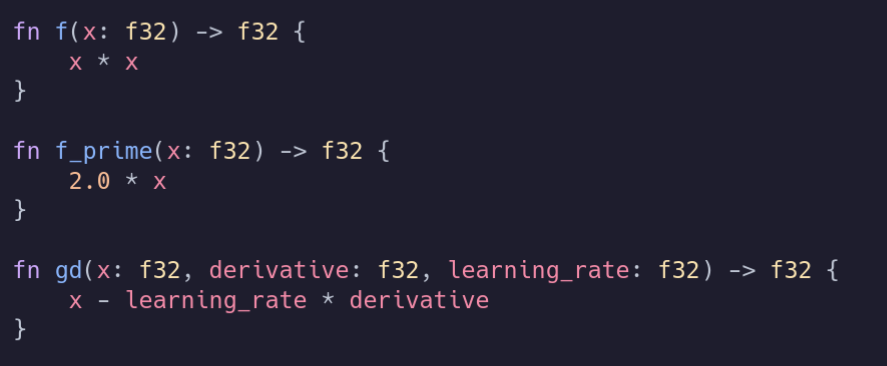
\includegraphics[width=1\linewidth]{impl.png}
        \subcaption{f, f\_prime and gd functions}
        \label{fig:enter-label}
    \end{subfigure}
    \begin{subfigure}{0.4\linewidth}
        \centering
        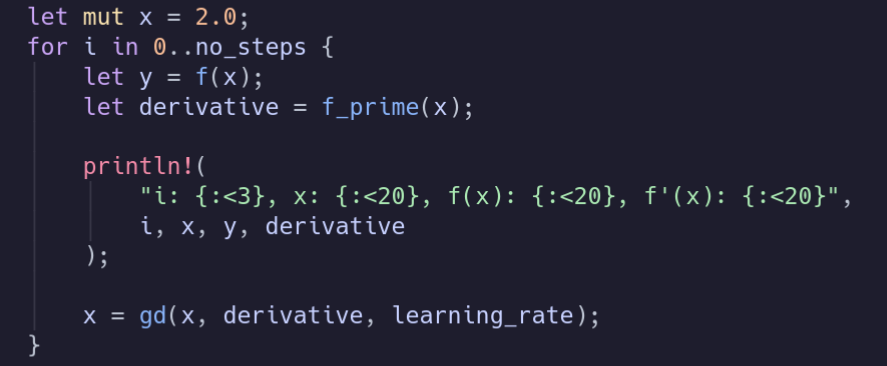
\includegraphics[width=1\linewidth]{impl2.png}
        \subcaption{Iteration code}
        \label{fig:enter-label}
    \end{subfigure}
    \caption{Gradient Descent implementation}
    \label{fig:enter-label}
\end{figure}

\begin{figure}[H]
    \centering
    
    \begin{subfigure}{0.3\linewidth}
        \centering
        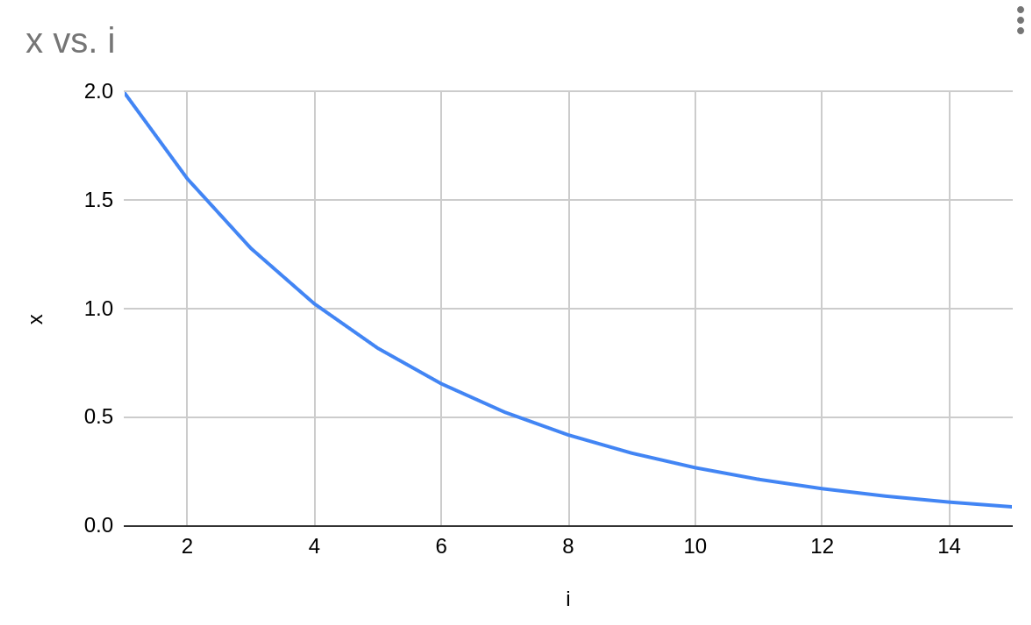
\includegraphics[width=\textwidth]{x.png}
        \subcaption{x}
        \label{fig:enter-label}
    \end{subfigure}

    \begin{subfigure}{0.3\textwidth}
        \centering
        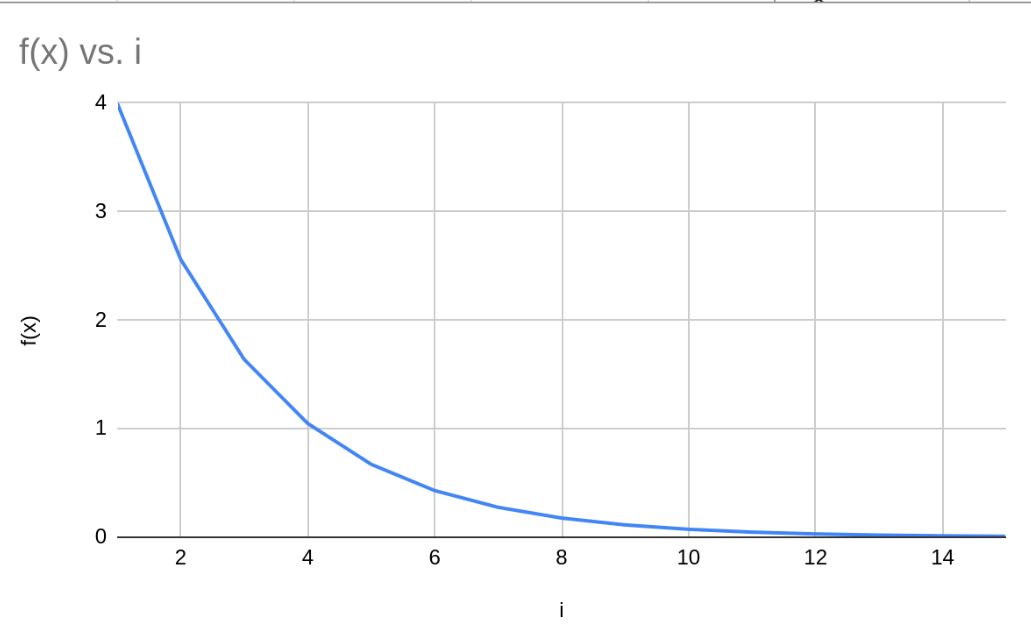
\includegraphics[width=\textwidth]{fx.png}
        \subcaption{f(x)}
        \label{fig:enter-label}
    \end{subfigure}
    
    \begin{subfigure}{0.3\linewidth}
        \centering
        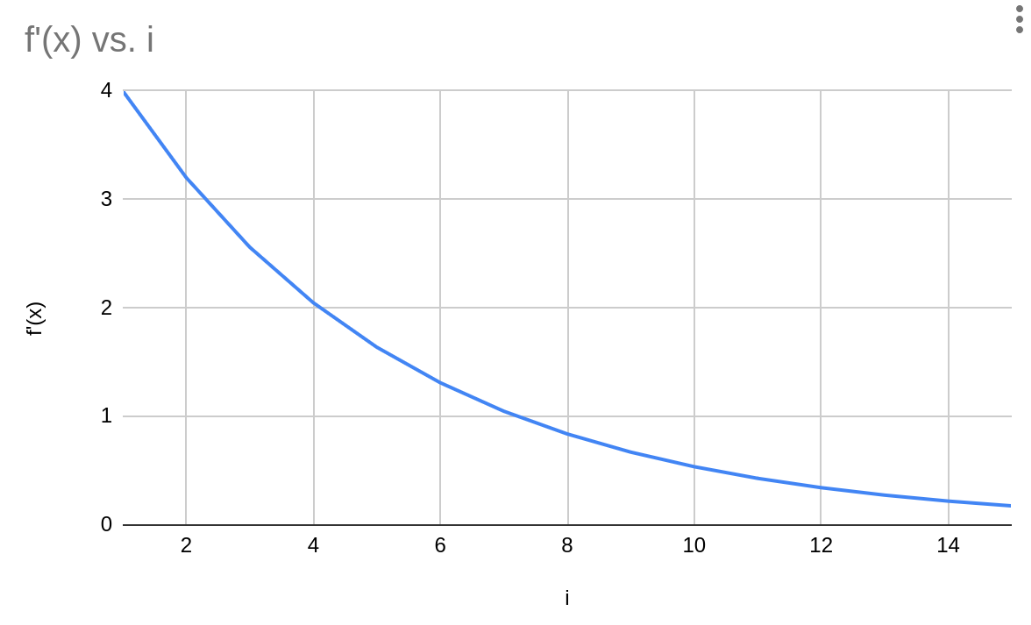
\includegraphics[width=\linewidth]{f_prime.png}
        \subcaption{f'(x)}
        \label{fig:enter-label}
    \end{subfigure}
    
    \caption{Good learning rate (0.1)}
    \label{fig:good}
\end{figure}


\begin{figure}
    \centering
    \begin{subfigure}{0.3\linewidth}
        \centering
        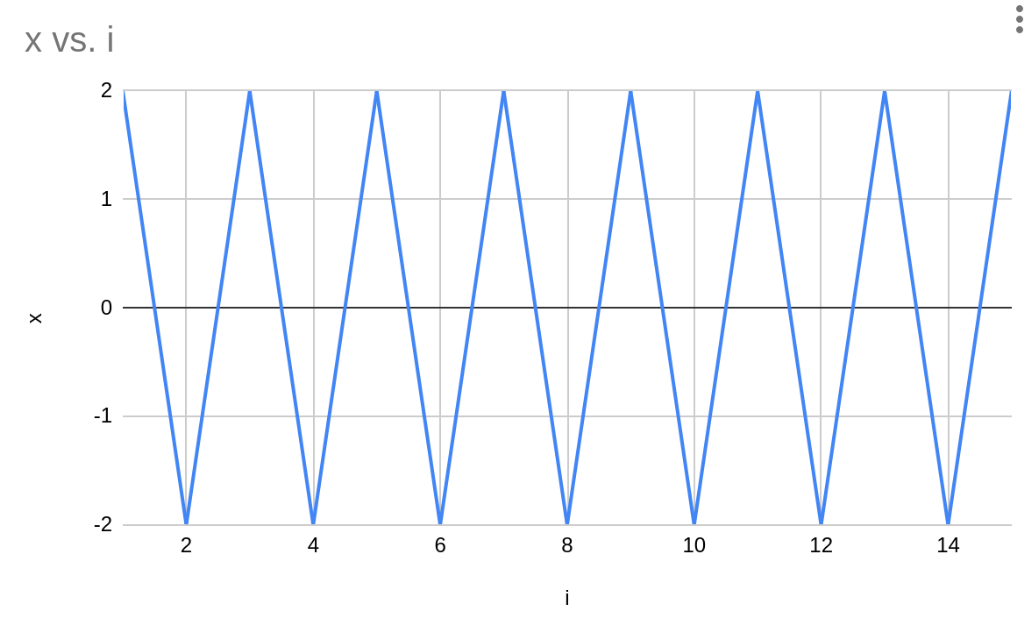
\includegraphics[width=\linewidth]{x_l.png}
        \caption{x}
        \label{fig:enter-label}
    \end{subfigure}
    
    \begin{subfigure}{0.3\linewidth}
        \centering
        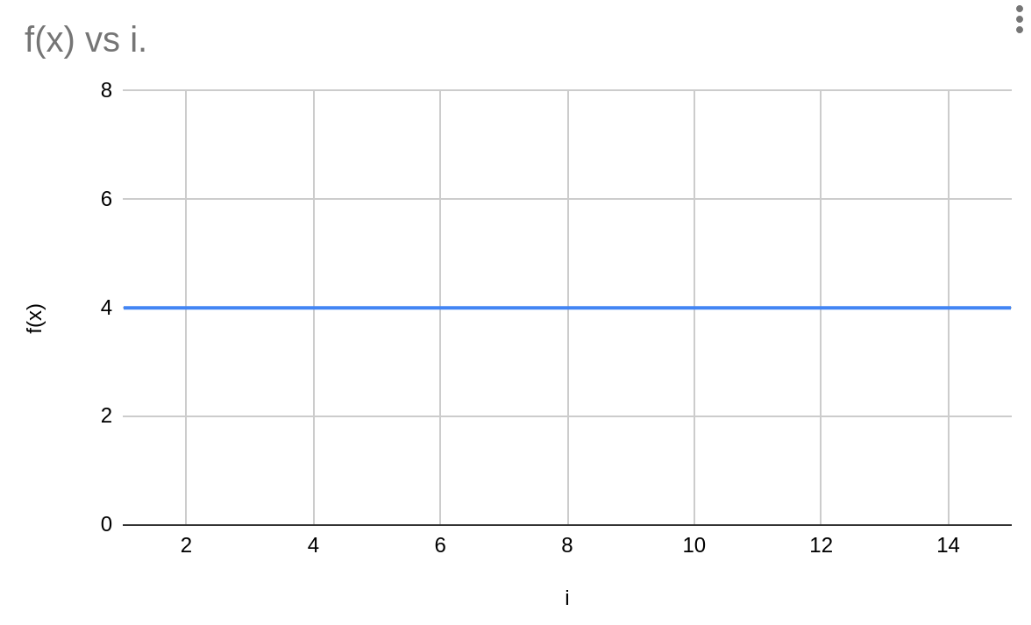
\includegraphics[width=\linewidth]{fx_l.png}
        \caption{f(x)}
        \label{fig:enter-label}
    \end{subfigure}
    
    \begin{subfigure}{0.3\linewidth}
        \centering
        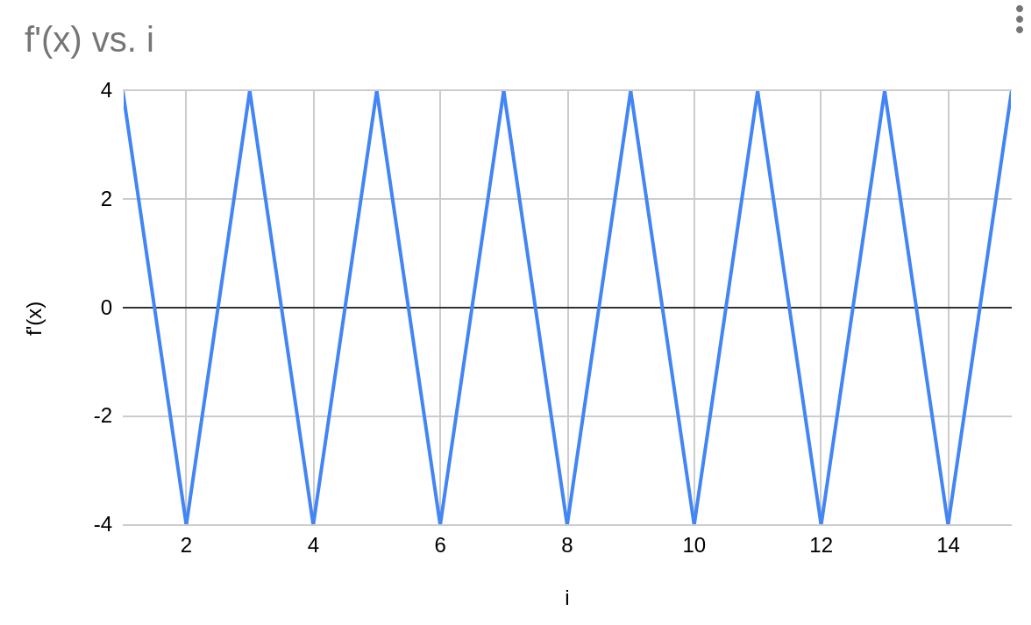
\includegraphics[width=\linewidth]{f_prime_l.png}
        \caption{f'(x)}
        \label{fig:enter-label}
    \end{subfigure}
    \caption{High learning rate (1)}
    \label{fig:enter-label}
\end{figure}


\begin{figure}
    \centering
    \begin{subfigure}{0.3\linewidth}
        \centering
        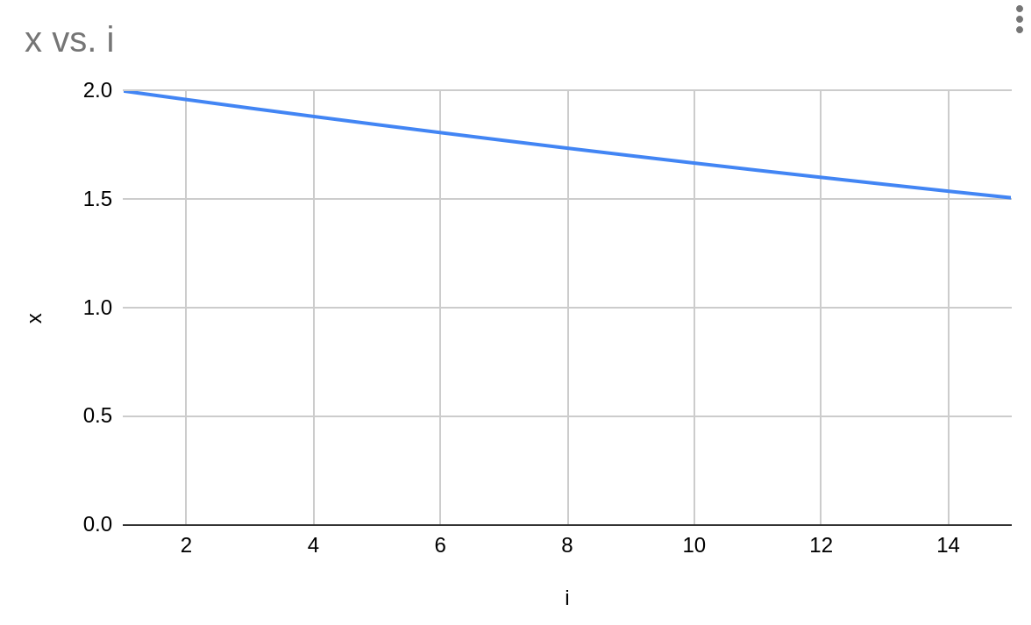
\includegraphics[width=\linewidth]{x_s.png}
        \caption{x}
        \label{fig:enter-label}
    \end{subfigure}
    
    \begin{subfigure}{0.3\linewidth}
        \centering
        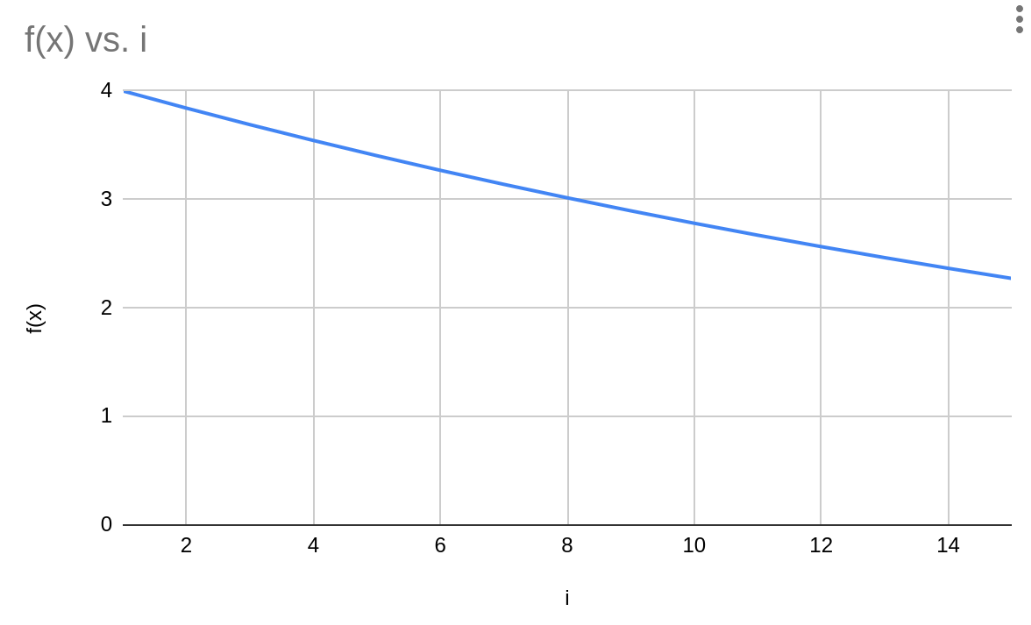
\includegraphics[width=\linewidth]{fx_s.png}
        \caption{f(x)}
        \label{fig:enter-label}
    \end{subfigure}
    
    \begin{subfigure}{0.3\linewidth}
        \centering
        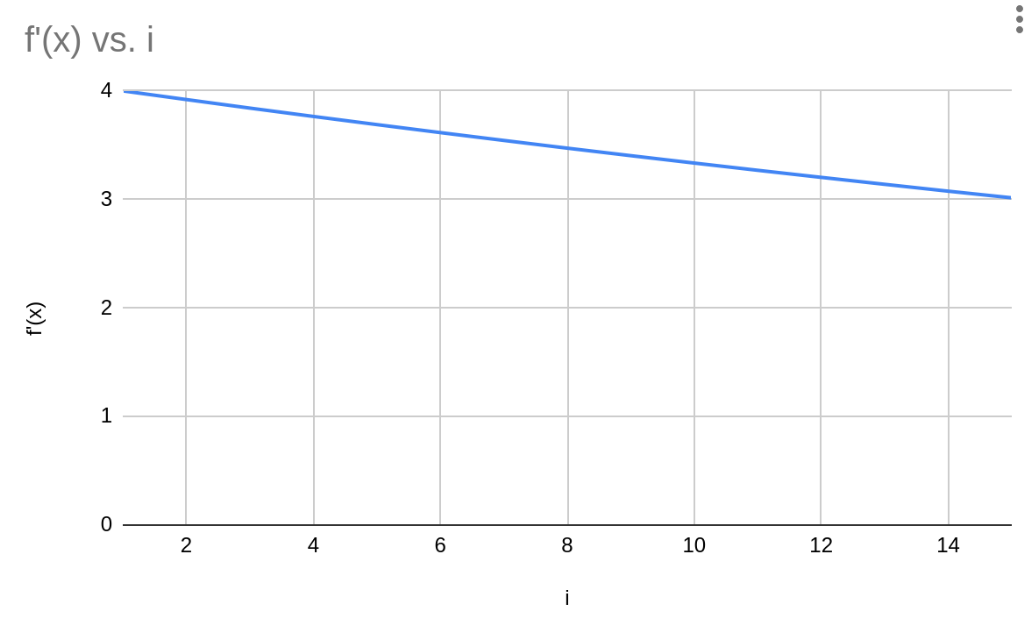
\includegraphics[width=\linewidth]{f_prime_s.png}
        \caption{f'(x)}
        \label{fig:enter-label}
    \end{subfigure}

    \caption{Too small learning rate (0.01)}
    \label{fig:enter-label}
\end{figure}

\begin{figure}
    \centering
    \begin{subfigure}{0.3\linewidth}
        \centering
        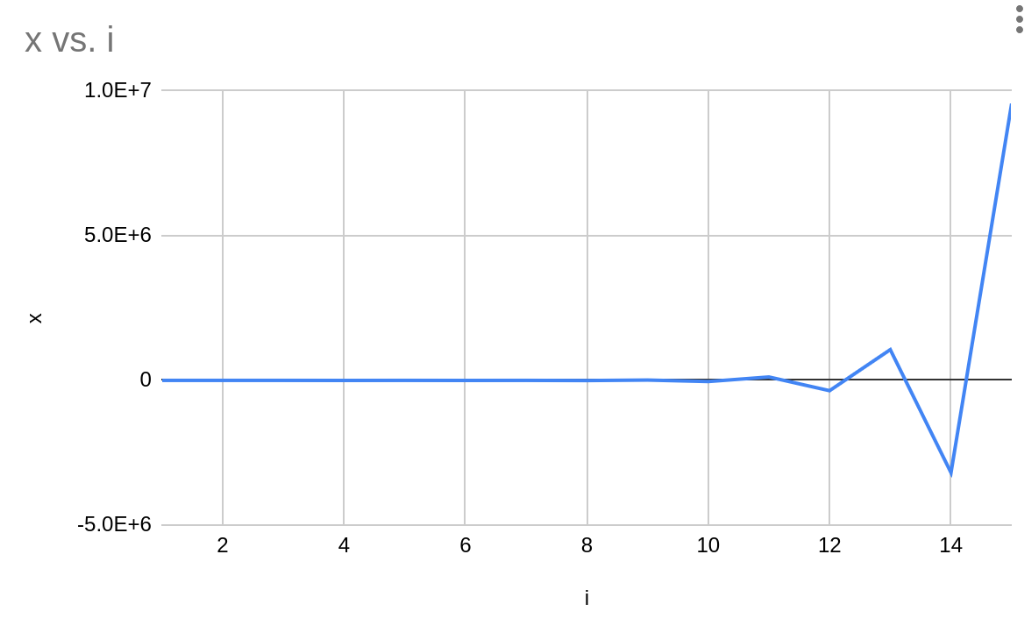
\includegraphics[width=\linewidth]{x_h.png}
        \caption{x}
        \label{fig:enter-label}
    \end{subfigure}
    
    
    \begin{subfigure}{0.3\linewidth}
        \centering
        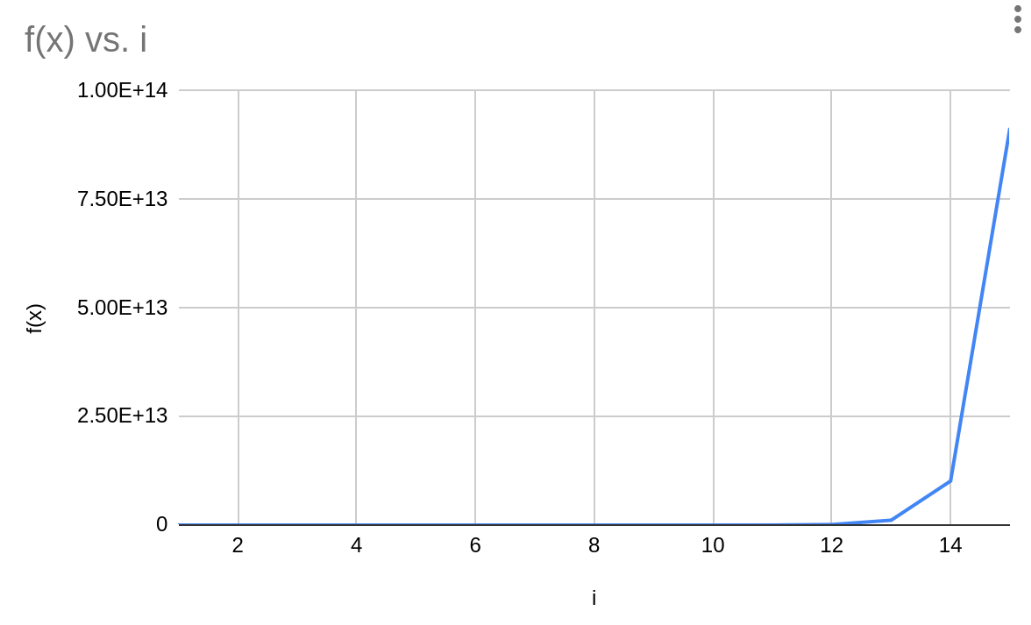
\includegraphics[width=\linewidth]{fx_h.png}
        \caption{f(x)}
        \label{fig:enter-label}
    \end{subfigure}
    
    \begin{subfigure}{0.3\linewidth}
        \centering
        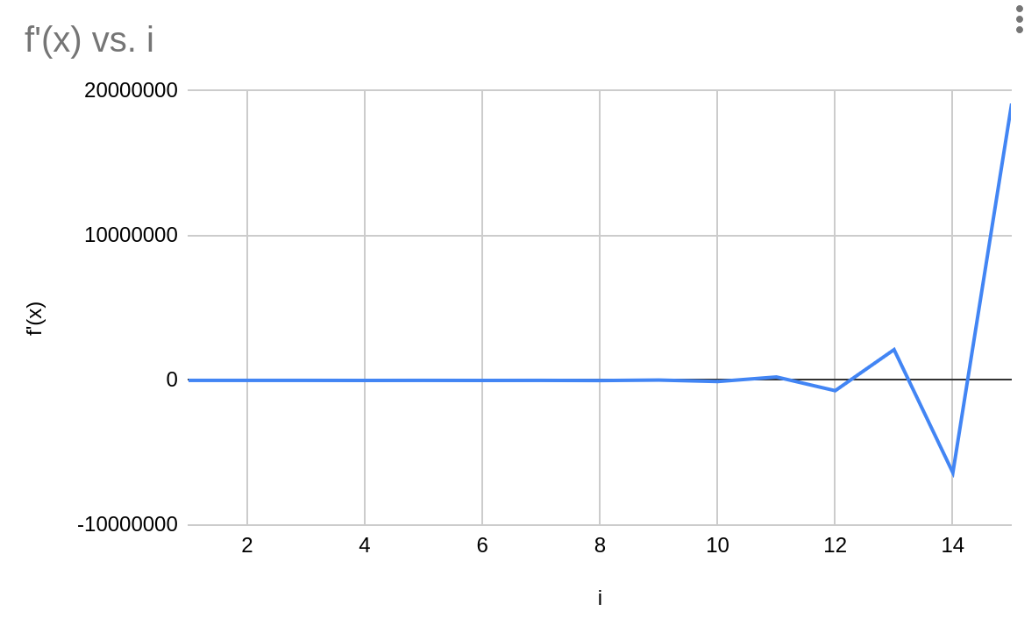
\includegraphics[width=\linewidth]{f_prime_h.png}
        \caption{f'(x)}
        \label{fig:enter-label}
    \end{subfigure}
    
    \caption{Hugh learning rate (2)}
    \label{fig:enter-label}
\end{figure}

\end{document}
